\documentclass[11pt,a4paper]{article}
\usepackage[a4paper,margin=2.5cm]{geometry}
\usepackage[T1]{fontenc}
\usepackage[utf8]{inputenc}
\usepackage[turkish]{babel}
\usepackage{lmodern}
\usepackage{microtype}
\usepackage[hidelinks]{hyperref}

\usepackage{amsmath,amssymb}
\usepackage{algorithm}
\usepackage{algpseudocode}

\usepackage{graphicx}
\usepackage{longtable}
\usepackage{makecell}
\bibliographystyle{plain}

\floatname{algorithm}{Algoritma}

\begin{document}
    \begin{titlepage}
  \centering

  \vspace*{1.5cm}

  {\LARGE\bfseries
    Walrus Optimizer (WO): Temel İlkeleri ve Matematiksel Modeli\par}

  \vspace{0.5cm}

  {\large
    PSO ve ACO ile Karşılaştırmalı Bir İnceleme\par}

  \vspace{1.5cm}

  {\large Luis Miguel Casañ González\par}

  \vfill

  {\small
    Karadeniz Teknik Üniversitesi\\
    İstatistik ve Bilgisayar Bilimleri Yüksek Lisans Programı\\
    Ders: Sürü Zekâsı\par}

  \vspace{0.5cm}

  {\normalsize 27 Ekim 2026\par}

  \vspace*{1.5cm}
\end{titlepage}

    \newpage
    \begin{abstract}
    Bu çalışmada, Walrus Optimizer (WO) algoritmasının temel ilkeleri ve
    matematiksel modeli incelenmektedir. Algoritmanın arama mekanizmaları
    açıklanmakta ve WO, Particle Swarm Optimization (PSO) ile Ant Colony
    Optimization (ACO) yöntemleriyle karşılaştırılmaktadır.
    \end{abstract}

    \noindent\textbf{Anahtar kelimeler:}
    Walrus Optimizer, sürü zekâsı, meta-sezgisel optimizasyon, PSO, ACO.

    \noindent\textbf{Kod deposu:}
    \href{https://github.com/lmcasan/metaheuristic-algorithms}{GitHub}

    \newpage
    \setcounter{section}{2}
    \section{Walrus Optimizer (WO)}
        % Biological Fundamentals
        \subsection{Biyolojik Temeller}

Walrus Optimizer (WO), morsaların yaşam biçimlerinden ve grup
davranışlarından esinlenen sürü zekâsı tabanlı bir meta-sezgisel
algoritmadır.

Morsalar, çoğunlukla Arktik çevresindeki soğuk denizlerde yaşayan ve
gruplar hâlinde hareket eden memelilerdir. Karada ve buz üzerinde
dinlenebilir, su altında besin arayabilirler. Üst dudaklarındaki hassas
bıyıklar çevreyi algılamalarına yardımcı olur; uzun köpek dişleri ise
savunma, deniz tabanındaki besinleri ortaya çıkarma ve buz üzerine
tırmanma gibi işlevler görür. Bu özellikler, WO'da kullanılan
mekanizmaların biyolojik arka planını açıklar; ancak algoritmadaki
matematiksel işlemler bu davranışların doğrudan biyolojik kopyaları
değil, optimizasyon amacıyla yapılmış soyutlamalardır.

\paragraph{Sosyal ve çevresel davranışlar.}
WO'nun dayandığı biyolojik gözlemler aşağıdaki şekilde özetlenebilir:

\begin{itemize}
    \item \textbf{Üreme döneminde alan seçimi:} Üreme döneminde erkek
    morsalar sahilde bölgeler edinir. Makalede, daha güçlü erkeklerin
    daha elverişli bölgeleri elde edebildiği ve bölgenin büyüklüğünün
    eşleştikleri dişi sayısıyla ilişkili olduğu belirtilir.

    \item \textbf{Besin arama ve bilgi paylaşımı:} Morsalar deniz
    tabanında besin ararken çevrelerinden yararlanır. Makale, onların
    ses yoluyla yön bulma ve besin bilgilerini diğer bireylerle paylaşma
    davranışlarına dikkat çeker.

    \item \textbf{Toplu savunma ve yardımlaşma:} Katil balina gibi
    tehditlerle karşılaştıklarında morsalar grup hâlinde savunma
    davranışı gösterebilir ve yaralanan bireylere yardım edebilir.
    Bu gözlem, tehlikeye karşı sürü üyelerinin birbirleriyle
    etkileşimini vurgular.

    \item \textbf{Göç ve dinlenme:} Morsalar çevresel koşullara ve
    yaşam döngülerine bağlı olarak hareket eder; karada veya buz
    üzerinde topluca dinlenebilir, suya girerek besin arayabilir.
\end{itemize}

WO, bu gözlemleri arama sürecinde farklı işlevleri olan mekanizmalar
olarak ele alır. Göç davranışı, arama ajanlarının çözüm uzayında yeni
bölgelere yönelmesini; besin arama, aday çözümlerin değerlendirilmesini
ve umut vadeden bölgelerde daha ayrıntılı arama yapılmasını temsil eder.
Üreme davranışı, başarılı çözümlerden yararlanarak yeni aday çözümler
oluşturma fikrine karşılık gelir. Dinlenme ve toplu davranışlar sürü
içindeki etkileşimleri, tehlikeden kaçınma ise arama sürecinde konum
değiştirerek yerel çözümlere aşırı bağlı kalma riskini azaltma fikrini
destekler.

Bu biyolojik analojiler, WO'da arama uzayını keşfetme
ile mevcut iyi çözümlerin çevresinde yoğunlaşma
arasında denge kurmak amacıyla kullanılır.
        % Mathematical model and algorithm
        \subsection{Matematiksel Model ve Algoritma}

WO, sürekli optimizasyon problemlerinde her bir
morsayı bir aday çözüm olarak ele alır. Bir morsanın konumu,
problemin karar değişkenlerinden oluşan bir vektördür. WO'nun amacı,
bu vektörleri yinelemeli olarak güncelleyerek amaç fonksiyonunu en
küçükleyen veya en büyükleyen çözümü bulmaktır.

\begin{equation}
    \min_{\mathbf{x}} f(\mathbf{x}),
    \max_{\mathbf{x}} f(\mathbf{x}):
    \qquad
    \mathbf{LB} \leq \mathbf{x} \leq \mathbf{UB},
    \label{eq:wo_problem}
\end{equation}

Burada $f(\mathbf{x})$ amaç fonksiyonunu, $\mathbf{LB}$ ve
$\mathbf{UB}$ ise karar değişkenlerinin alt ve üst sınırlarını
göstermektedir. En büyükleme problemleri, amaç fonksiyonunun işareti
değiştirilerek en küçükleme problemine dönüştürülebilir.

\subsubsection{Başlangıç popülasyonu}

Popülasyon, $N$ adet morsadan oluşur. $d$ karar değişkeni bulunan bir
problemde, $i$'inci morsanın konumu
$\mathbf{X}_i=(X_{i,1},X_{i,2},\ldots,X_{i,d})$ biçimindedir.
Başlangıç konumları, arama uzayına düzgün dağılımlı rastgele sayılar
kullanılarak yerleştirilir:

\begin{equation}
    X_{i,j}^{0}
    =
    LB_j + u_{i,j}(UB_j-LB_j),
    \qquad
    u_{i,j}\sim\mathcal{U}(0,1),
    \label{eq:wo_initialization}
\end{equation}

Burada $i=1,\ldots,N$ ve $j=1,\ldots,d$'dir. Başlangıç popülasyonunda
morsaların yüzde 90'ı yetişkin, yüzde 10'u yavru olarak kabul edilir.
Yetişkin morsalar kendi içinde eşit sayıda erkek ve dişi bireyden
oluşur. Her aday çözümün uygunluğu $f(\mathbf{X}_i)$ hesaplanır ve
en iyi çözüm $\mathbf{X}_{\mathrm{best}}$ olarak kaydedilir.

\subsubsection{Tehlike ve güvenlik sinyalleri}

WO'da sürünün davranışını seçmek için tehlike ve güvenlik sinyalleri
kullanılır. $t$ mevcut yinelemeyi, $T$ ise en fazla yineleme sayısını
göstersin. Tehlike sinyali aşağıdaki gibi tanımlanır:

\begin{align}
    \alpha_t &= 1-\frac{t}{T}, \label{eq:wo_alpha}\\
    A_t &= 2\alpha_t, \label{eq:wo_A}\\
    R_t &= 2r_1-1, \qquad r_1\sim\mathcal{U}(0,1), \label{eq:wo_R}\\
    D_t &= A_tR_t \label{eq:wo_danger}
\end{align}

Güvenlik sinyali ise başka bir düzgün dağılımlı rastgele sayı ile
hesaplanır:

\begin{equation}
    S_t=r_2,
    \qquad
    r_2\sim\mathcal{U}(0,1).
    \label{eq:wo_safety}
\end{equation}

Yineleme ilerledikçe $\alpha_t$ azalır. WO, bu sinyalleri kullanarak
arama davranışını göç, dinlenme, besin arama ve kaçış aşamalarından
birine yönlendirir.

\subsubsection{Göç: keşif aşaması}

Tehlike sinyalinin mutlak değeri en az 1 olduğunda sürü göç davranışı
gösterir. Algoritmik açıdan bu davranış, aday çözümlerin arama
uzayında yeni bölgelere yönlendirilmesini sağlar. $m$ ve $n$, sürüden
rastgele seçilen iki farklı bireyi göstermek üzere:

\begin{align}
    \mathbf{X}_i^{t+1}
    &=
    \mathbf{X}_i^t+\mathbf{Migration\_step}_t,
    \label{eq:wo_migration}\\
    \mathbf{Migration\_step}_t
    &=
    \left(\mathbf{X}_m^t-\mathbf{X}_n^t\right)
    \beta_t r_3^2,
    \qquad r_3\sim\mathcal{U}(0,1),
    \label{eq:wo_migration_step}\\
    \beta_t
    &=
    1-
    \frac{1}{
        1+\exp\left(
            -10\frac{t-T/2}{T}
        \right)
    }.
    \label{eq:wo_beta}
\end{align}

Burada $\mathbf{Migration\_step}_t$ göç adımını, $\beta_t$ ise bu adımın büyüklüğünü
kontrol eden katsayıyı ifade eder. $\beta_t$ yinelemeler boyunca
azalarak aramanın başlangıcında daha geniş, ilerleyen aşamalarda ise
daha sınırlı hareketler yapılmasına katkıda bulunur.

\subsubsection{Üreme: sömürü aşaması}

$|D_t|<1$ olduğunda WO üreme aşamasına geçer. Bu aşamada güvenlik
sinyali, morsaların kıyıda dinlenme davranışını mı yoksa su altında
besin arama davranışını mı izleyeceğini belirler.

\paragraph{Kıyıda dinlenme davranışı.}

$S_t\geq 0.5$ olduğunda dinlenme davranışı uygulanır. Bu davranışta
morsalar erkek, dişi ve yavru bireyler olarak ele alınır ve her grubun
konumu farklı biçimde güncellenir.

Erkek bireylerin konumları Halton dizisi kullanılarak arama uzayına
yeniden dağıtılır. Bir uygulamada bu işlem aşağıdaki biçimde
gerçekleştirilebilir:

\begin{equation}
    X_{i,j}^{t+1}
    =
    LB_j+h_{i,j}^{t}(UB_j-LB_j),
    \qquad h_{i,j}^{t}\in[0,1],
    \label{eq:wo_male_halton}
\end{equation}

Burada $h_{i,j}^{t}$, Halton dizisinin $j$'inci boyutundaki değeridir.
Bu işlem erkek bireylerin farklı bölgeleri örneklemesini ve
popülasyon çeşitliliğinin korunmasını amaçlar.

Dişi bireylerin konumları hem eş olarak kabul edilen erkek bireyden
hem de sürünün o ana kadarki en iyi çözümünden etkilenir:

\begin{equation}
\begin{aligned}
    \mathbf{F}_i^{t+1}
    ={}& \mathbf{F}_i^t
    +\alpha_t\left(\mathbf{Migration\_step}_i^t-\mathbf{F}_i^t\right)\\
    &+(1-\alpha_t)
    \left(\mathbf{X}_{\mathrm{best}}^t-\mathbf{F}_i^t\right).
\end{aligned}
\label{eq:wo_female}
\end{equation}

Burada $\mathbf{F}_i^t$ dişi bireyin, $\mathbf{Migration\_step}_i^t$ ise onunla
eşleştirilen erkek bireyin konumudur. $\alpha_t$ azaldıkça erkek
bireyin etkisi azalır; en iyi çözümün etkisi artar.

Yavru bireyler için önce güvenli referans konumu hesaplanır:

\begin{align}
    \mathbf{O}_i^t
    &=
    \mathbf{X}_{\mathrm{best}}^t
    +\mathbf{J}_i^t\odot\mathbf{LF},
    \label{eq:wo_safety_position}\\
    \mathbf{J}_i^{t+1}
    &=
    \left(\mathbf{O}_i^t-\mathbf{J}_i^t\right)P,
    \qquad P\sim\mathcal{U}(0,1).
    \label{eq:wo_juvenile}
\end{align}

Burada $\mathbf{J}_i^t$ yavru bireyin mevcut konumu, $P$ rastgele
rahatsızlık katsayısı, $\odot$ bileşen bazında çarpım ve $\mathbf{LF}$
Lévy dağılımına dayalı hareket vektörüdür. Lévy hareketi aşağıdaki
biçimde modellenir:

\begin{align}
    LF
    &=
    0.05\frac{x}{|y|^{1/\lambda}},
    \qquad
    x\sim\mathcal{N}(0,\sigma_x^2),
    \quad
    y\sim\mathcal{N}(0,\sigma_y^2),
    \label{eq:wo_levy}\\
    \sigma_x
    &=
    \left[
        \frac{
            \Gamma(1+\lambda)\sin(\pi\lambda/2)
        }{
            \Gamma((1+\lambda)/2)\lambda 2^{(\lambda-1)/2}
        }
    \right]^{1/\lambda},
    \qquad
    \sigma_y=1,
    \qquad
    \lambda=1.5.
    \label{eq:wo_levy_sigma}
\end{align}

$\Gamma(\cdot)$, Gamma fonksiyonudur. Lévy hareketinin uzun adımlar
üretebilmesi, yavru bireylerin çevredeki çözümlerden uzaklaşarak farklı
bölgeleri örneklemesine olanak tanır.

\paragraph{Su altında besin arama davranışı.}

$S_t<0.5$ olduğunda algoritma besin arama davranışına geçer. Bu
davranış, tehlike sinyaline göre kaçış veya toplanma olarak ikiye
ayrılır.

$|D_t|\geq 0.5$ olduğunda kaçış davranışı uygulanır:

\begin{equation}
    \mathbf{X}_i^{t+1}
    =
    \mathbf{X}_i^t R_t
    -
    \left|
        \mathbf{X}_{\mathrm{best}}^t-\mathbf{X}_i^t
    \right|r_4^2,
    \qquad r_4\sim\mathcal{U}(0,1).
    \label{eq:wo_fleeing}
\end{equation}

Mutlak değer, vektörlerde bileşen bazında alınır. Bu güncelleme,
bireyin mevcut konumunu değiştirerek sürünün bulunduğu bölgeden
uzaklaşmasını sağlar.

$|D_t|<0.5$ olduğunda toplanma davranışı uygulanır:

\begin{align}
    \mathbf{X}_i^{t+1}
    &=
    \frac{\mathbf{X}_1+\mathbf{X}_2}{2},
    \label{eq:wo_gathering}\\
    \mathbf{X}_1
    &=
    \mathbf{X}_{\mathrm{best}}^t
    -a_1b_1
    \left|
        \mathbf{X}_{\mathrm{best}}^t-\mathbf{X}_i^t
    \right|,
    \label{eq:wo_gather_x1}\\
    \mathbf{X}_2
    &=
    \mathbf{X}_{\mathrm{second}}^t
    -a_2b_2
    \left|
        \mathbf{X}_{\mathrm{second}}^t-\mathbf{X}_i^t
    \right|,
    \label{eq:wo_gather_x2}\\
    a_k
    &=
    \beta_t r_5-\beta_t,
    \qquad
    b_k=\tan(\theta_k),
    \qquad
    r_5\sim\mathcal{U}(0,1),
    \quad
    \theta_k\in[0,\pi],
    \quad k\in\{1,2\}.
    \label{eq:wo_gather_coefficients}
\end{align}

Burada $\mathbf{X}_{\mathrm{second}}^t$, o anki popülasyondan seçilen
ikinci bir bireyin konumunu temsil eder. $\mathbf{X}_1$ ve
$\mathbf{X}_2$, en iyi ve ikinci birey çevresinde oluşturulan iki
aday yönelimdir; yeni konum bu iki yönelimin ortalamasıyla elde edilir.
$\tan(\theta_k)$ fonksiyonu $\theta_k=\pi/2$ noktasında tanımsız
olduğundan, sayısal uygulamada bu noktaya çok yakın değerler
örneklenmemelidir.

\subsubsection{WO algoritmasının sözde kodu}

Algoritmanın temel karar akışı Algoritma~\ref{alg:wo} içinde
özetlenmiştir. Her yinelemede önce tehlike sinyali kontrol edilir.
Tehlike yüksekse göç uygulanır; aksi durumda güvenlik sinyali dinlenme
ve besin arama davranışları arasında seçim yapar.

\begin{algorithm}[htbp]
\caption{Walrus Optimizer (WO)}
\label{alg:wo}
\begin{algorithmic}[1]
\Require Amaç fonksiyonu $f$, alt ve üst sınırlar $\mathbf{LB}$ ve
         $\mathbf{UB}$, popülasyon büyüklüğü $N$, en fazla yineleme $T$
\Ensure En iyi çözüm $\mathbf{X}_{\mathrm{best}}$ ve amaç fonksiyonu değeri

\State $\mathbf{X}\gets$ Denklem~\eqref{eq:wo_initialization}'e göre popülasyonu başlat
\State Bireyleri yetişkin, erkek, dişi ve yavru gruplarına ayır
\State $f(\mathbf{X}_i)$ değerlerini hesapla
\State $\mathbf{X}_{\mathrm{best}}\gets$ mevcut en iyi birey
\For{$t=0$ \textbf{to} $T-1$}
    \State $D_t\gets$ Denklem~\eqref{eq:wo_danger}'e göre tehlike sinyalini hesapla
    \State $S_t\gets$ Denklem~\eqref{eq:wo_safety}'e göre güvenlik sinyalini hesapla
    \If{$|D_t|\geq 1$}
        \State Her bireyin konumunu göç denklemleri
               \eqref{eq:wo_migration}--\eqref{eq:wo_beta} ile güncelle
    \Else
        \If{$S_t\geq 0.5$}
            \State Erkek bireyleri Halton dizisi ile yeniden dağıt
            \State Dişi bireyleri Denklem~\eqref{eq:wo_female} ile güncelle
            \State Yavru bireyleri Denklem~\eqref{eq:wo_juvenile} ile güncelle
        \Else
            \If{$|D_t|\geq 0.5$}
                \State Her bireyin konumunu kaçış davranışına
                       göre, Denklem~\eqref{eq:wo_fleeing} ile güncelle
            \Else
                \State Her bireyin konumunu toplanma davranışına
                       göre, Denklem~\eqref{eq:wo_gathering} ile güncelle
            \EndIf
        \EndIf
    \EndIf
    \State Sınırları aşan konumları problem kısıtlarına göre düzelt
    \State Yeni bireylerin amaç fonksiyonu değerlerini hesapla
    \State $\mathbf{X}_{\mathrm{best}}$ değerini güncelle
\EndFor
\State \Return $\mathbf{X}_{\mathrm{best}}$
\end{algorithmic}
\end{algorithm}

        % Comparison
        \begingroup
\shorthandoff{=}
\renewcommand{\tablename}{Tablo}
\renewcommand{\figurename}{Şekil}
\graphicspath{{src/figures/}{figures/}}

\section{Sonuçların analizi}
\label{sec:benchmark-analysis}

\subsection{Nitel analiz}
WO'nun nitel sonuçları, standart kıyaslama fonksiyonları kullanılarak
değerlendirilmiştir. İncelenen kıyaslama kümesi, fonksiyonların optimizasyon
yapısına ve boyut özelliklerine göre üç gruba ayrılmıştır:
tek tepeli (unimodal), çok tepeli (multimodal) ve sabit boyutlu çok tepeli
(fixed-dimension multimodal) fonksiyonlar. Makale \cite{han2024walrus}’te önerilen 
bu sınıflandırmaya göre F1–F7 fonksiyonları tek tepeli, F8–F13 fonksiyonları çok tepeli, 
F14–F23 fonksiyonları ise sabit boyutlu çok tepeli grupta yer almaktadır.
\cite{han2024walrus}.

Tek tepeli fonksiyonlar tek bir küresel optimuma sahiptir. Bu nedenle,
algoritmanın optimuma doğru ilerlemesi ve çözüm kalitesini iyileştirmesi
hakkında bilgi verirler. Çok tepeli fonksiyonlar birden fazla yerel optimum
içerir; bu fonksiyonlar algoritmanın yerel çözümlere erken yakınsama
eğilimini ve arama uzayının farklı bölgelerini keşfetme yeteneğini incelemek
için kullanılır. Sabit boyutlu çok tepeli fonksiyonlarda ise değişken sayısı
fonksiyonun tanımıyla belirlenmiştir ve keyfî olarak artırılamaz. Bu grup,
algoritmanın belirli boyutlara sahip, daha karmaşık ve çok tepeli arama
uzaylarındaki davranışını değerlendirmeye olanak tanır.

Sonuçlar dört ölçüt üzerinden incelenmiştir: arama geçmişi, ilk ajanın
yörüngesi, popülasyonun ortalama uygunluğu ve yakınsama eğrisi
\cite{han2024walrus}. Arama geçmişi, ajanların iterasyonlar boyunca ziyaret
ettiği bölgeleri; ilk ajanın yörüngesi, tek bir ajanın hareketini; ortalama
uygunluk, popülasyonun genel performansını; yakınsama eğrisi ise iterasyonlar
boyunca elde edilen en iyi çözümün değişimini gösterir. Böylece WO'nun hem
arama uzayını keşfetme davranışı hem de çözümleri iyileştirme süreci nitel
olarak değerlendirilebilir.

\begin{figure}[htbp]
\centering
\begin{minipage}[t]{0.48\textwidth}\centering\small
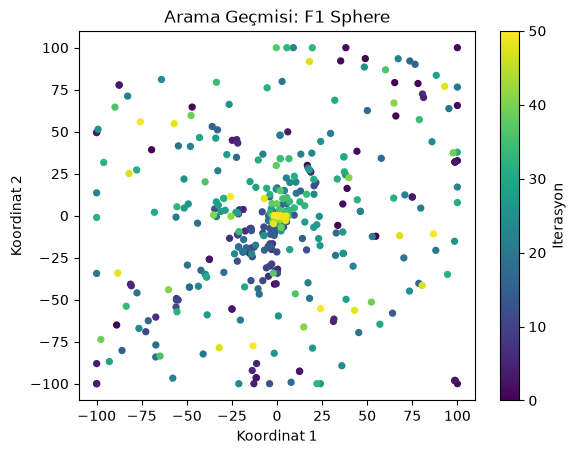
\includegraphics[width=\linewidth]{F1/search_history.png}
\end{minipage}\hfill
\begin{minipage}[t]{0.48\textwidth}\centering\small 
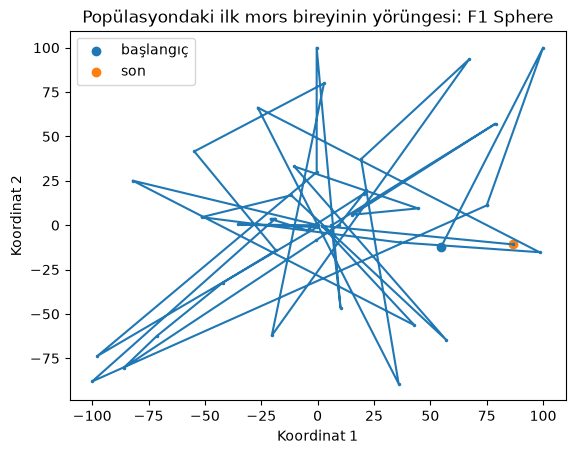
\includegraphics[width=\linewidth]{F1/first_walrus_trajectory.png}
\end{minipage}\par\medskip
\begin{minipage}[t]{0.48\textwidth}\centering\small
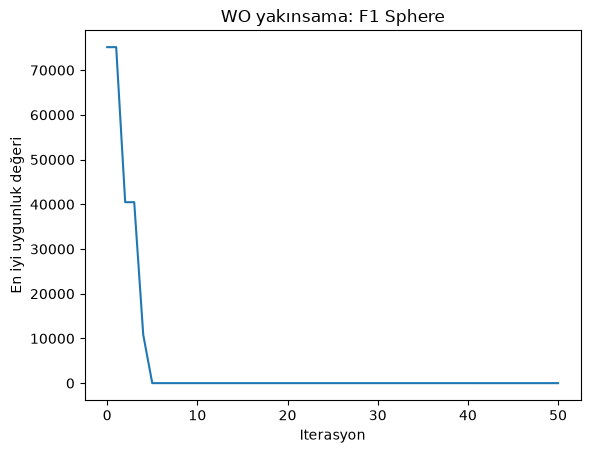
\includegraphics[width=\linewidth]{F1/convergence.png}
\end{minipage}\hfill
\begin{minipage}[t]{0.48\textwidth}\centering\small
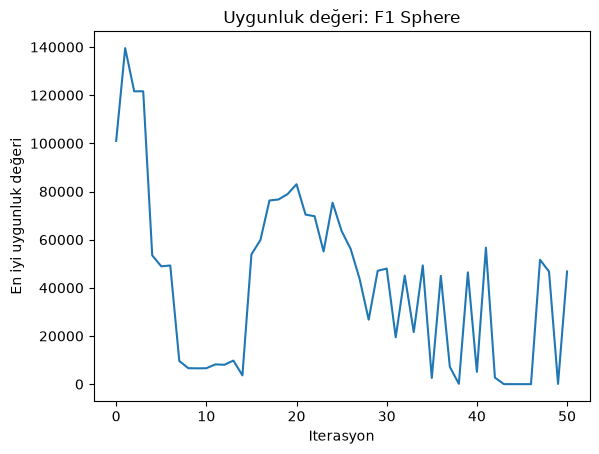
\includegraphics[width=\linewidth]{F1/average_fitness.png}
\end{minipage}
\caption{WO'nun F1 Sphere fonksiyonundaki nitel arama sonuçları.}
\label{fig:wo-f1-qualitative}
\end{figure}

Şekil~\ref{fig:wo-f1-qualitative}'de arama geçmişinin önemli bir bölümü optimum olan orijinin çevresinde 
yoğunlaşırken arama uzayına yayılan sıçramalar da görülmektedir. İlk morsun yörüngesi geniş ve ani hareketler içerir; 
yörüngenin son noktası optimuma yakın değildir. Buna karşın, yakınsama eğrisi en iyi uygunluğun ilk birkaç yinelemede sıfıra 
yaklaştığını ve sonrasında korunduğunu gösterir. Popülasyonun ortalama uygunluğu ise yinelemeler boyunca belirgin biçimde 
dalgalanır. 

\begin{figure}[htbp]
\centering
\begin{minipage}[t]{0.48\textwidth}\centering\small
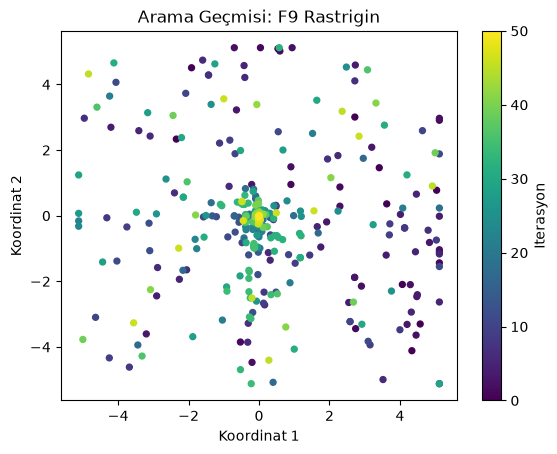
\includegraphics[width=\linewidth]{F9/search_history.png}
\end{minipage}\hfill
\begin{minipage}[t]{0.48\textwidth}\centering\small 
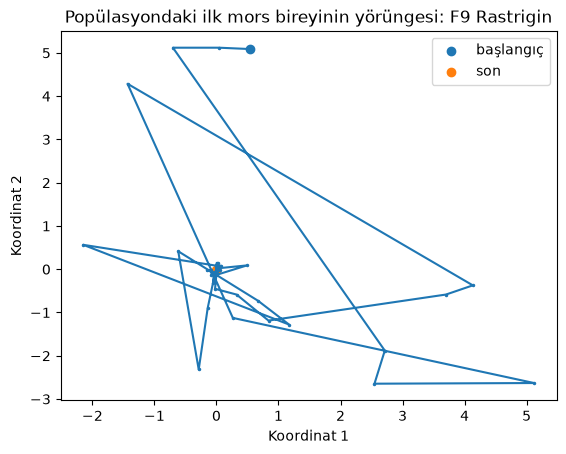
\includegraphics[width=\linewidth]{F9/first_walrus_trajectory.png}
\end{minipage}\par\medskip
\begin{minipage}[t]{0.48\textwidth}\centering\small
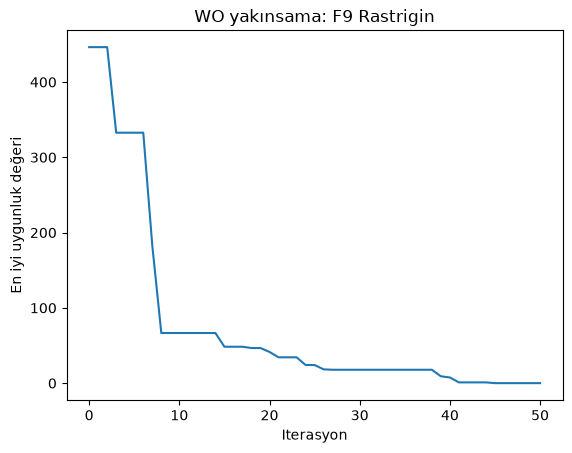
\includegraphics[width=\linewidth]{F9/convergence.png}
\end{minipage}\hfill
\begin{minipage}[t]{0.48\textwidth}\centering\small
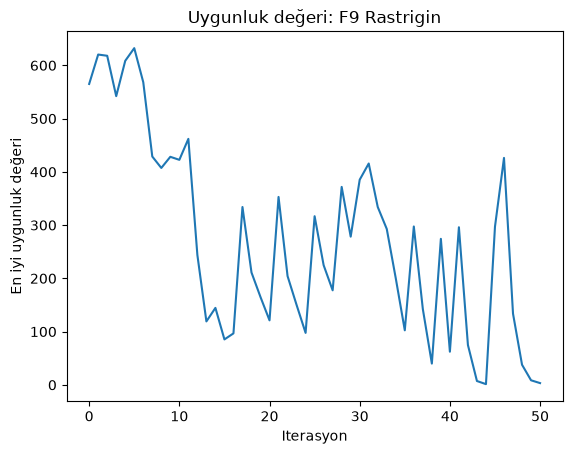
\includegraphics[width=\linewidth]{F9/average_fitness.png}
\end{minipage}
\caption{WO'nun F9 Rastrigin fonksiyonundaki nitel arama sonuçları.}
\label{fig:wo-f9-qualitative}
\end{figure}

F9 Rastrigin çok sayıda yerel optimum içerir. Şekil~\ref{fig:wo-f9-qualitative}'de noktaların geniş bir alana yayıldıktan sonra orijin çevresinde de yoğunlaştığı görülür. Yakınsama eğrisi en iyi değerin yinelemeler ilerledikçe kademeli olarak azaldığını ve çalıştırmanın son bölümünde sıfıra yaklaştığını gösterir. İlk morsun yörüngesi ve ortalama uygunluk eğrisi ise büyük sıçramalar ve dalgalanmalar sergiler. Bu nedenle arama geçmişindeki merkezî yoğunlaşma, her ajanın yerel optimumlardan kaçtığını tek başına kanıtlamaz.

\begin{figure}[htbp]
\centering
\begin{minipage}[t]{0.48\textwidth}\centering\small
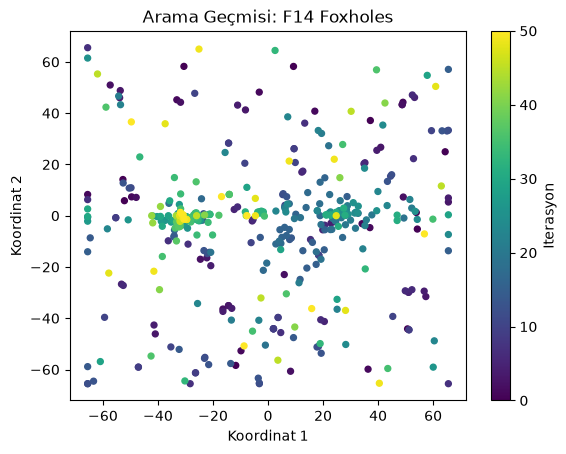
\includegraphics[width=\linewidth]{F14/search_history.png}
\end{minipage}\hfill
\begin{minipage}[t]{0.48\textwidth}\centering\small
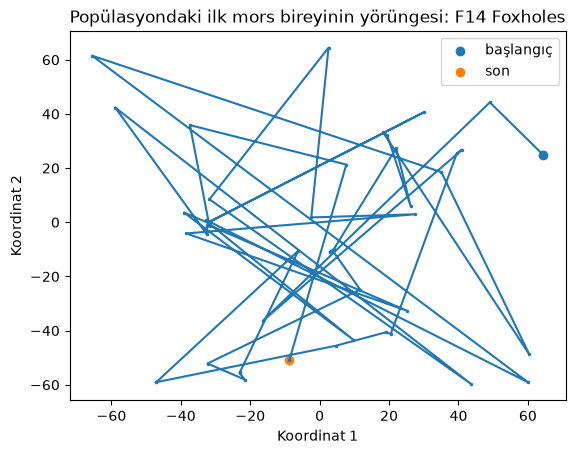
\includegraphics[width=\linewidth]{F14/first_walrus_trajectory.png}
\end{minipage}\par\medskip
\begin{minipage}[t]{0.48\textwidth}\centering\small
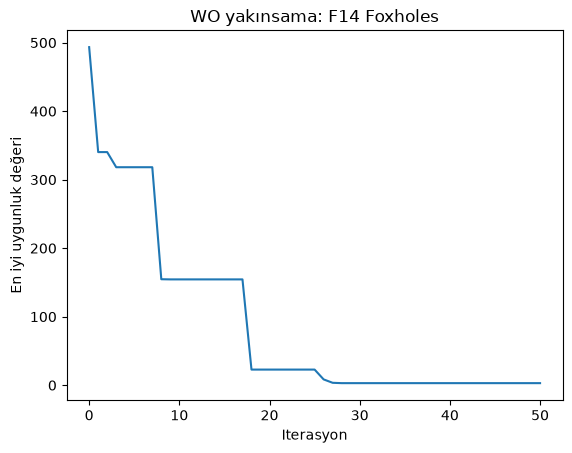
\includegraphics[width=\linewidth]{F14/convergence.png}
\end{minipage}\hfill
\begin{minipage}[t]{0.48\textwidth}\centering\small
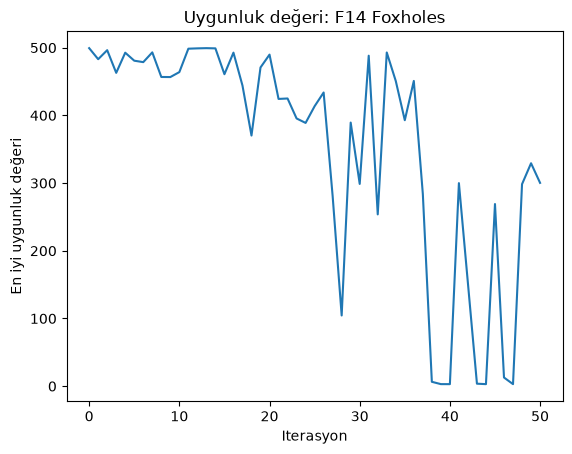
\includegraphics[width=\linewidth]{F14/average_fitness.png}
\end{minipage}
\caption{WO'nun F14 Foxholes fonksiyonundaki nitel arama sonuçları.}
\label{fig:wo-f14-qualitative}
\end{figure}

Şekil~\ref{fig:wo-f14-qualitative}’te, F14 Foxholes için arama geçmişi, ajanların arama uzayının geniş bir bölümünü ziyaret ettiğini ve bazı 
bölgelerde kümelenmeler oluştuğunu göstermektedir. İlk morsun yörüngesi geniş ve düzensiz hareketler içerir; 
başlangıç noktası yaklaşık \((65,25)\), son noktası ise yaklaşık \((-9,-50)\)’dir. Bu yörünge, ilk morsun optimuma 
yakınsadığını göstermemektedir. Buna karşılık yakınsama eğrisi, bulunan en iyi uygunluk değerinin ilk yaklaşık 
27 yinelemede belirgin biçimde azaldığını ve sonrasında sıfıra yakın kaldığını göstermektedir. Popülasyonun uygunluk 
değerindeki büyük dalgalanmalar ise bireylerin aynı hızda kararlı hâle gelmediğine işaret eder. Dolayısıyla en iyi 
çözümün hızla iyileşmesi, ilk morsun veya popülasyonun tamamının optimuma yakınsadığı anlamına gelmez.

Han ve arkadaşları makaledeki seçili testlerde, yinelemeler ilerledikçe ilk ajanın hareket genliğinin azaldığını, 
aramanın daha elverişli bölgelere yöneldiğini ve ortalama uygunluğun düştüğünü bildirmiştir \cite{han2024walrus}. 
Buradaki grafiklerde en iyi çözüm eğrileri bu iyileşme eğilimiyle uyumludur; ancak ilk morsun yörüngeleri ve 
popülasyon ortalaması her üç fonksiyonda da belirgin hareketlilik göstermektedir.

\subsection{Nicel analiz}

\paragraph{Toplu karşılaştırma.}
Her fonksiyon için 100 çalıştırmanın ortalama uygunluk değerleri esas alınarak
algoritmalar sıralanmıştır. Buna göre WO, POS'u 23 fonksiyonun 16'sında, ACO'yu
ise 15'inde geçmiştir. ACO da POS'tan 18 fonksiyonda daha düşük ortalama
uygunluk elde etmiştir. Tablo~\ref{tab:overall-rank-results}, ortalama uygunluk
temelindeki ikili W/T/L sonuçlarını göstermektedir.

\begin{table}[htbp]
\centering
\small
\caption{Ortalama uygunluk değerlerine göre ikili W/T/L sonuçları ve Friedman ortalama sıra değerleri.}
\label{tab:overall-rank-results}
\begin{tabular}{@{}lrrrr@{}}
\hline
\textbf{Karşılaştırma} & \textbf{W} & \textbf{T} & \textbf{L} & \textbf{Fonksiyon sayısı} \\
\hline
WO--POS & 16 & 0 & 7 & 23 \\
WO--ACO & 15 & 0 & 8 & 23 \\
ACO--POS & 18 & 0 & 5 & 23 \\
\hline
\end{tabular}
\vspace{0.8em}
\begin{tabular}{@{}lrr@{}}
\hline
\textbf{Algoritma} & \textbf{Friedman ortalama sırası} & \textbf{Genel sıra} \\
\hline
WO & 1.652 & 1 \\
ACO & 1.870 & 2 \\
POS & 2.478 & 3 \\
\hline
\end{tabular}
\end{table}
Friedman testi, algoritmalar arasında genel bir fark bulunduğunu göstermiştir ($\chi^2(2)=8.435$, $p=0.0147$). Friedman testi ikili farkları tek başına belirlemediğinden, algoritma çiftleri için post-hoc test yapılmadan ikili istatistiksel anlamlılık iddiasında bulunulmamıştır.


\small
\setlength{\tabcolsep}{3pt}
\renewcommand{\arraystretch}{1.12}
\begin{longtable}{@{}p{2.25cm}p{4.25cm}p{4.25cm}p{4.25cm}@{}}
\caption{WO, POS ve ACO algoritmalarının 23 kıyaslama fonksiyonundaki sonuçları. Süreler 100 çalıştırmadaki medyan saniye değeridir.}\label{tab:all-benchmark-results}\\
\hline
\textbf{Fonksiyon} & \textbf{WO} & \textbf{POS} & \textbf{ACO} \\
\hline
\endfirsthead
\multicolumn{4}{c}{\tablename\ \thetable{} -- devamı}\\
\hline
\textbf{Fonksiyon} & \textbf{WO} & \textbf{POS} & \textbf{ACO} \\
\hline
\endhead
\hline
\multicolumn{4}{r}{Devamı sonraki sayfada}\\
\endfoot
\hline
\endlastfoot
\multicolumn{4}{@{}l}{\textbf{Tek tepeli fonksiyonlar (F1--F7)}}\\
F1 Sphere & \makecell[l]{En iyi: $4.794\times 10^{-10}$\\ En kötü: $96.65$\\ Ortalama: $3.078$\\ Std. sapma: $12.42$\\ Medyan süre: $0.01379\,\mathrm{s}$} & \makecell[l]{En iyi: $1.725\times 10^{4}$\\ En kötü: $5.567\times 10^{4}$\\ Ortalama: $3.67\times 10^{4}$\\ Std. sapma: $8553$\\ Medyan süre: $0.005513\,\mathrm{s}$} & \makecell[l]{En iyi: $2771$\\ En kötü: $2.069\times 10^{4}$\\ Ortalama: $1.128\times 10^{4}$\\ Std. sapma: $3735$\\ Medyan süre: $0.01193\,\mathrm{s}$} \\
F2 Schwefel 2.22 & \makecell[l]{En iyi: $7.989\times 10^{-7}$\\ En kötü: $2.772$\\ Ortalama: $0.2129$\\ Std. sapma: $0.4244$\\ Medyan süre: $0.01567\,\mathrm{s}$} & \makecell[l]{En iyi: $90.45$\\ En kötü: $2.192\times 10^{9}$\\ Ortalama: $8.319\times 10^{7}$\\ Std. sapma: $3.658\times 10^{8}$\\ Medyan süre: $0.008007\,\mathrm{s}$} & \makecell[l]{En iyi: $26.93$\\ En kötü: $6441$\\ Ortalama: $185.4$\\ Std. sapma: $711.3$\\ Medyan süre: $0.01178\,\mathrm{s}$} \\
F3 Schwefel 1.2 & \makecell[l]{En iyi: $3.204\times 10^{-9}$\\ En kötü: $9740$\\ Ortalama: $237.8$\\ Std. sapma: $1125$\\ Medyan süre: $0.008233\,\mathrm{s}$} & \makecell[l]{En iyi: $4.442\times 10^{4}$\\ En kötü: $1.24\times 10^{5}$\\ Ortalama: $7.943\times 10^{4}$\\ Std. sapma: $1.84\times 10^{4}$\\ Medyan süre: $0.003734\,\mathrm{s}$} & \makecell[l]{En iyi: $4.152\times 10^{4}$\\ En kötü: $1.22\times 10^{5}$\\ Ortalama: $7.589\times 10^{4}$\\ Std. sapma: $1.631\times 10^{4}$\\ Medyan süre: $0.006859\,\mathrm{s}$} \\
F4 Schwefel 2.21 & \makecell[l]{En iyi: $1.504\times 10^{-7}$\\ En kötü: $11.28$\\ Ortalama: $0.7973$\\ Std. sapma: $1.714$\\ Medyan süre: $0.006398\,\mathrm{s}$} & \makecell[l]{En iyi: $66.54$\\ En kötü: $96.86$\\ Ortalama: $88.51$\\ Std. sapma: $5.607$\\ Medyan süre: $0.002547\,\mathrm{s}$} & \makecell[l]{En iyi: $73.54$\\ En kötü: $96.86$\\ Ortalama: $90.94$\\ Std. sapma: $4.142$\\ Medyan süre: $0.005817\,\mathrm{s}$} \\
F5 Rosenbrock & \makecell[l]{En iyi: $28.95$\\ En kötü: $1.056\times 10^{5}$\\ Ortalama: $1127$\\ Std. sapma: $1.056\times 10^{4}$\\ Medyan süre: $0.008323\,\mathrm{s}$} & \makecell[l]{En iyi: $2.617\times 10^{7}$\\ En kötü: $2.649\times 10^{8}$\\ Ortalama: $9.89\times 10^{7}$\\ Std. sapma: $4.607\times 10^{7}$\\ Medyan süre: $0.00439\,\mathrm{s}$} & \makecell[l]{En iyi: $1.88\times 10^{6}$\\ En kötü: $7.884\times 10^{7}$\\ Ortalama: $2.912\times 10^{7}$\\ Std. sapma: $1.57\times 10^{7}$\\ Medyan süre: $0.007724\,\mathrm{s}$} \\
F6 Step & \makecell[l]{En iyi: $0$\\ En kötü: $42$\\ Ortalama: $2.5$\\ Std. sapma: $7.132$\\ Medyan süre: $0.007244\,\mathrm{s}$} & \makecell[l]{En iyi: $1.712\times 10^{4}$\\ En kötü: $6.123\times 10^{4}$\\ Ortalama: $3.575\times 10^{4}$\\ Std. sapma: $8683$\\ Medyan süre: $0.003149\,\mathrm{s}$} & \makecell[l]{En iyi: $3249$\\ En kötü: $2.34\times 10^{4}$\\ Ortalama: $1.181\times 10^{4}$\\ Std. sapma: $3561$\\ Medyan süre: $0.006282\,\mathrm{s}$} \\
F7 Quartic & \makecell[l]{En iyi: $0.005393$\\ En kötü: $4.336\times 10^{5}$\\ Ortalama: $4633$\\ Std. sapma: $4.337\times 10^{4}$\\ Medyan süre: $0.009031\,\mathrm{s}$} & \makecell[l]{En iyi: $7.385\times 10^{8}$\\ En kötü: $8.591\times 10^{9}$\\ Ortalama: $4.258\times 10^{9}$\\ Std. sapma: $1.681\times 10^{9}$\\ Medyan süre: $0.004956\,\mathrm{s}$} & \makecell[l]{En iyi: $3.154\times 10^{8}$\\ En kötü: $3.779\times 10^{9}$\\ Ortalama: $1.272\times 10^{9}$\\ Std. sapma: $6.532\times 10^{8}$\\ Medyan süre: $0.008021\,\mathrm{s}$} \\
\multicolumn{4}{@{}l}{\textbf{Çok tepeli fonksiyonlar (F8--F13)}}\\
F8 Schwefel 2.26 & \makecell[l]{En iyi: $-7789$\\ En kötü: $-2134$\\ Ortalama: $-3460$\\ Std. sapma: $928.5$\\ Medyan süre: $0.007317\,\mathrm{s}$} & \makecell[l]{En iyi: $-7344$\\ En kötü: $-4190$\\ Ortalama: $-5726$\\ Std. sapma: $715.7$\\ Medyan süre: $0.003529\,\mathrm{s}$} & \makecell[l]{En iyi: $-5105$\\ En kötü: $-2390$\\ Ortalama: $-3392$\\ Std. sapma: $559.3$\\ Medyan süre: $0.006649\,\mathrm{s}$} \\
F9 Rastrigin & \makecell[l]{En iyi: $3.675\times 10^{-9}$\\ En kötü: $146$\\ Ortalama: $2.879$\\ Std. sapma: $15.5$\\ Medyan süre: $0.007749\,\mathrm{s}$} & \makecell[l]{En iyi: $288$\\ En kötü: $451$\\ Ortalama: $375.9$\\ Std. sapma: $36.58$\\ Medyan süre: $0.003985\,\mathrm{s}$} & \makecell[l]{En iyi: $242.6$\\ En kötü: $413.7$\\ Ortalama: $324.3$\\ Std. sapma: $27.82$\\ Medyan süre: $0.007093\,\mathrm{s}$} \\
F10 Ackley & \makecell[l]{En iyi: $1.338\times 10^{-5}$\\ En kötü: $3.691$\\ Ortalama: $0.2538$\\ Std. sapma: $0.607$\\ Medyan süre: $0.01048\,\mathrm{s}$} & \makecell[l]{En iyi: $17.38$\\ En kötü: $20.68$\\ Ortalama: $20.1$\\ Std. sapma: $0.5688$\\ Medyan süre: $0.006594\,\mathrm{s}$} & \makecell[l]{En iyi: $12.35$\\ En kötü: $20.71$\\ Ortalama: $18.42$\\ Std. sapma: $1.916$\\ Medyan süre: $0.009975\,\mathrm{s}$} \\
F11 Griewank & \makecell[l]{En iyi: $1.181\times 10^{-10}$\\ En kötü: $11.63$\\ Ortalama: $0.561$\\ Std. sapma: $1.231$\\ Medyan süre: $0.009479\,\mathrm{s}$} & \makecell[l]{En iyi: $128.7$\\ En kötü: $531.7$\\ Ortalama: $320$\\ Std. sapma: $77.4$\\ Medyan süre: $0.005419\,\mathrm{s}$} & \makecell[l]{En iyi: $52.5$\\ En kötü: $220.4$\\ Ortalama: $106.5$\\ Std. sapma: $31.11$\\ Medyan süre: $0.008727\,\mathrm{s}$} \\
F12 Penalized 1 & \makecell[l]{En iyi: $0.1766$\\ En kötü: $5.392$\\ Ortalama: $1.157$\\ Std. sapma: $0.5741$\\ Medyan süre: $0.01374\,\mathrm{s}$} & \makecell[l]{En iyi: $2.866\times 10^{7}$\\ En kötü: $5.203\times 10^{8}$\\ Ortalama: $1.879\times 10^{8}$\\ Std. sapma: $9.329\times 10^{7}$\\ Medyan süre: $0.009702\,\mathrm{s}$} & \makecell[l]{En iyi: $4.059\times 10^{6}$\\ En kötü: $3.828\times 10^{8}$\\ Ortalama: $7.592\times 10^{7}$\\ Std. sapma: $6.763\times 10^{7}$\\ Medyan süre: $0.0133\,\mathrm{s}$} \\
F13 Penalized 2 & \makecell[l]{En iyi: $2.369$\\ En kötü: $50.6$\\ Ortalama: $3.915$\\ Std. sapma: $4.902$\\ Medyan süre: $0.0126\,\mathrm{s}$} & \makecell[l]{En iyi: $7.835\times 10^{7}$\\ En kötü: $1.176\times 10^{9}$\\ Ortalama: $3.999\times 10^{8}$\\ Std. sapma: $2.215\times 10^{8}$\\ Medyan süre: $0.008618\,\mathrm{s}$} & \makecell[l]{En iyi: $1.806\times 10^{7}$\\ En kötü: $6.201\times 10^{8}$\\ Ortalama: $1.528\times 10^{8}$\\ Std. sapma: $1.018\times 10^{8}$\\ Medyan süre: $0.01188\,\mathrm{s}$} \\
\multicolumn{4}{@{}l}{\textbf{Sabit boyutlu çok tepeli fonksiyonlar (F14--F23)}}\\
F14 Foxholes & \makecell[l]{En iyi: $0.998$\\ En kötü: $16.44$\\ Ortalama: $6.535$\\ Std. sapma: $3.444$\\ Medyan süre: $0.00935\,\mathrm{s}$} & \makecell[l]{En iyi: $0.998$\\ En kötü: $20.21$\\ Ortalama: $3.849$\\ Std. sapma: $3.865$\\ Medyan süre: $0.006552\,\mathrm{s}$} & \makecell[l]{En iyi: $0.998$\\ En kötü: $16.45$\\ Ortalama: $5.353$\\ Std. sapma: $3.605$\\ Medyan süre: $0.009232\,\mathrm{s}$} \\
F15 Kowalik & \makecell[l]{En iyi: $0.00592$\\ En kötü: $0.1316$\\ Ortalama: $0.03691$\\ Std. sapma: $0.02265$\\ Medyan süre: $0.008102\,\mathrm{s}$} & \makecell[l]{En iyi: $0.005437$\\ En kötü: $0.1285$\\ Ortalama: $0.0585$\\ Std. sapma: $0.03518$\\ Medyan süre: $0.005234\,\mathrm{s}$} & \makecell[l]{En iyi: $0.004373$\\ En kötü: $0.09887$\\ Ortalama: $0.02601$\\ Std. sapma: $0.02265$\\ Medyan süre: $0.008094\,\mathrm{s}$} \\
F16 Six-hump Camel & \makecell[l]{En iyi: $-1.032$\\ En kötü: $-0.9906$\\ Ortalama: $-1.028$\\ Std. sapma: $0.00759$\\ Medyan süre: $0.004477\,\mathrm{s}$} & \makecell[l]{En iyi: $-1.032$\\ En kötü: $-1.026$\\ Ortalama: $-1.031$\\ Std. sapma: $0.0007045$\\ Medyan süre: $0.001905\,\mathrm{s}$} & \makecell[l]{En iyi: $-1.032$\\ En kötü: $-0.2155$\\ Ortalama: $-1.023$\\ Std. sapma: $0.08161$\\ Medyan süre: $0.00468\,\mathrm{s}$} \\
F17 Branin & \makecell[l]{En iyi: $0.3979$\\ En kötü: $0.6619$\\ Ortalama: $0.4146$\\ Std. sapma: $0.04435$\\ Medyan süre: $0.004559\,\mathrm{s}$} & \makecell[l]{En iyi: $0.3979$\\ En kötü: $12.72$\\ Ortalama: $0.6505$\\ Std. sapma: $1.522$\\ Medyan süre: $0.002001\,\mathrm{s}$} & \makecell[l]{En iyi: $0.3979$\\ En kötü: $0.3979$\\ Ortalama: $0.3979$\\ Std. sapma: $4.873\times 10^{-7}$\\ Medyan süre: $0.004659\,\mathrm{s}$} \\
F18 Goldstein-Price & \makecell[l]{En iyi: $3$\\ En kötü: $3.993$\\ Ortalama: $3.107$\\ Std. sapma: $0.184$\\ Medyan süre: $0.005224\,\mathrm{s}$} & \makecell[l]{En iyi: $3$\\ En kötü: $84.94$\\ Ortalama: $11.56$\\ Std. sapma: $24.66$\\ Medyan süre: $0.002675\,\mathrm{s}$} & \makecell[l]{En iyi: $3$\\ En kötü: $86.1$\\ Ortalama: $8.591$\\ Std. sapma: $17.84$\\ Medyan süre: $0.005251\,\mathrm{s}$} \\
F19 Hartmann 3D & \makecell[l]{En iyi: $-3.862$\\ En kötü: $-2.986$\\ Ortalama: $-3.768$\\ Std. sapma: $0.1447$\\ Medyan süre: $0.008336\,\mathrm{s}$} & \makecell[l]{En iyi: $-3.863$\\ En kötü: $-2.664$\\ Ortalama: $-3.816$\\ Std. sapma: $0.1672$\\ Medyan süre: $0.005525\,\mathrm{s}$} & \makecell[l]{En iyi: $-3.863$\\ En kötü: $-1.001$\\ Ortalama: $-3.834$\\ Std. sapma: $0.2862$\\ Medyan süre: $0.008116\,\mathrm{s}$} \\
F20 Hartmann 6D & \makecell[l]{En iyi: $-3.307$\\ En kötü: $-2.194$\\ Ortalama: $-3.108$\\ Std. sapma: $0.1753$\\ Medyan süre: $0.008287\,\mathrm{s}$} & \makecell[l]{En iyi: $-3.322$\\ En kötü: $-1.255$\\ Ortalama: $-3.039$\\ Std. sapma: $0.4329$\\ Medyan süre: $0.005498\,\mathrm{s}$} & \makecell[l]{En iyi: $-3.322$\\ En kötü: $-3.191$\\ Ortalama: $-3.277$\\ Std. sapma: $0.05792$\\ Medyan süre: $0.008248\,\mathrm{s}$} \\
F21 Shekel 5 & \makecell[l]{En iyi: $-9.559$\\ En kötü: $-1.73$\\ Ortalama: $-4.558$\\ Std. sapma: $1.557$\\ Medyan süre: $0.009906\,\mathrm{s}$} & \makecell[l]{En iyi: $-10.14$\\ En kötü: $-0.4973$\\ Ortalama: $-5.507$\\ Std. sapma: $3.252$\\ Medyan süre: $0.007176\,\mathrm{s}$} & \makecell[l]{En iyi: $-10.15$\\ En kötü: $-2.196$\\ Ortalama: $-5.276$\\ Std. sapma: $3.529$\\ Medyan süre: $0.009805\,\mathrm{s}$} \\
F22 Shekel 7 & \makecell[l]{En iyi: $-10.13$\\ En kötü: $-1.957$\\ Ortalama: $-4.403$\\ Std. sapma: $1.216$\\ Medyan süre: $0.009915\,\mathrm{s}$} & \makecell[l]{En iyi: $-10.4$\\ En kötü: $-0.9116$\\ Ortalama: $-4.93$\\ Std. sapma: $3.078$\\ Medyan süre: $0.007203\,\mathrm{s}$} & \makecell[l]{En iyi: $-10.4$\\ En kötü: $-1.838$\\ Ortalama: $-6.751$\\ Std. sapma: $3.695$\\ Medyan süre: $0.009829\,\mathrm{s}$} \\
F23 Shekel 10 & \makecell[l]{En iyi: $-10.12$\\ En kötü: $-1.718$\\ Ortalama: $-4.478$\\ Std. sapma: $1.651$\\ Medyan süre: $0.009745\,\mathrm{s}$} & \makecell[l]{En iyi: $-10.49$\\ En kötü: $-1.46$\\ Ortalama: $-4.733$\\ Std. sapma: $3.1$\\ Medyan süre: $0.007126\,\mathrm{s}$} & \makecell[l]{En iyi: $-10.54$\\ En kötü: $-1.809$\\ Ortalama: $-6.635$\\ Std. sapma: $3.9$\\ Medyan süre: $0.01003\,\mathrm{s}$} \\
\end{longtable}
\endgroup


    \newpage
    \bibliography{src/references}
\end{document}